%----------------------------------------------------------------------------------------
%  PACKAGES AND CONFIGURATION
%----------------------------------------------------------------------------------------

\documentclass{rapport}
\usepackage{geometry}
\usepackage{fancyhdr} % For custom headers
\usepackage{lastpage} % To determine the last page for the footer
\usepackage{float}
\usepackage{extramarks} % For headers and footers
\usepackage[most]{tcolorbox} % For problem answer sections
\usepackage{graphicx} % For inserting images
\usepackage{xcolor} % For link coloring
\usepackage[hidelinks]{hyperref} % For URL links (no box or color name) 

%Ce que moi(Alban) ai rajouté comme package
\usepackage{comment} 
\usepackage{multicol} % Pour les colonnes
\usepackage{listings}
\usepackage{courier}
\usepackage{subcaption}

\definecolor{backcolour}{RGB}{47,47,47}
\definecolor{violet}{RGB}{200,20,200}
\definecolor{codegreen}{rgb}{0,0.6,0}
\definecolor{codegray}{rgb}{0.5,0.5,0.5}
\definecolor{marron}{RGB}{150,100,70}
\definecolor{red2}{RGB}{207,43,58}
\definecolor{bordeaux}{RGB}{74,31,30}
\lstdefinestyle{mystyle}{
    language=Python,
    basicstyle=\tiny\ttfamily
    backgroundcolor=\color{backcolour},   
    commentstyle=\color{codegreen},
    keywordstyle=\color{violet},
    numberstyle=\tiny\color{codegray},
    stringstyle=\color{red},
    literate={,}{{\textcolor{red}{,}}}1
             {;}{{\textcolor{red}{;}}}1,
    basicstyle=\ttfamily\footnotesize,
    breakatwhitespace=false,         
    breaklines=true,                 
    captionpos=b,                    
    keepspaces=true,                 
    numbers=left,                    
    numbersep=5pt,                  
    showspaces=false,                
    showstringspaces=false,
    showtabs=false,                  
    tabsize=2,
    literate=
  {á}{{\'a}}1 {é}{{\'e}}1 {í}{{\'i}}1 {ó}{{\'o}}1 {ú}{{\'u}}1
  {Á}{{\'A}}1 {É}{{\'E}}1 {Í}{{\'I}}1 {Ó}{{\'O}}1 {Ú}{{\'U}}1
  {à}{{\`a}}1 {è}{{\`e}}1 {ì}{{\`i}}1 {ò}{{\`o}}1 {ù}{{\`u}}1
  {À}{{\`A}}1 {È}{{\'E}}1 {Ì}{{\`I}}1 {Ò}{{\`O}}1 {Ù}{{\`U}}1
  {ä}{{\"a}}1 {ë}{{\"e}}1 {ï}{{\"i}}1 {ö}{{\"o}}1 {ü}{{\"u}}1
  {Ä}{{\"A}}1 {Ë}{{\"E}}1 {Ï}{{\"I}}1 {Ö}{{\"O}}1 {Ü}{{\"U}}1
  {â}{{\^a}}1 {ê}{{\^e}}1 {î}{{\^i}}1 {ô}{{\^o}}1 {û}{{\^u}}1
  {Â}{{\^A}}1 {Ê}{{\^E}}1 {Î}{{\^I}}1 {Ô}{{\^O}}1 {Û}{{\^U}}1
  {œ}{{\oe}}1 {Œ}{{\OE}}1 {æ}{{\ae}}1 {Æ}{{\AE}}1 {ß}{{\ss}}1
  {ű}{{\H{u}}}1 {Ű}{{\H{U}}}1 {ő}{{\H{o}}}1 {Ő}{{\H{O}}}1
  {ç}{{\c c}}1 {Ç}{{\c C}}1 {ø}{{\o}}1 {å}{{\r a}}1 {Å}{{\r A}}1
  {€}{{\EUR}}1 {£}{{\pounds}}1
}

\title{TS229}
\begin{document}

%----------- Informations du rapport ---------
\logo{images/logo_em.jpg}
\unif{École nationale supérieure d'électronique, informatique, télécommunications, mathématiques et mécanique de Bordeaux}
\titre{Lecture de code-barres par lancers aléatoires de rayons}
\cours{Département Télécom} %Nom du cours
\sujet{TS225 : Projet Images} %Nom du sujet
\enseignant{Marc \textsc{DONIAS}}
\eleves{Elisa \textsc{Chien} \\
		Alban \textsc{Oberti} \\
		Tierno-Alpha \textsc{Tall} \\
		David \textsc{Yan} 
		}

%----------------------------------------------------------------------------------------
%   TITLE PAGE
%----------------------------------------------------------------------------------------
\fairemarges %Afficher les marges
\fairepagedegarde %Créer la page de garde
\newpage
\tabledematieres %Créer la table de matières
\newpage
% ------------------------------------------------ %

\section{Introduction}

\section{Algorithmes}

\subsection{Phase 1 : Détection du code barre}
\subsection{Phase 2 : Lecture du code barre}

La phase précédente a permis de récupérer un ensemble de couple de points représentant des rayons. 
Pour chaque couple de points, nous déterminons d'une part les 13 valeurs du code barre, et d'autre part, s'il est valide ou non.

\subsubsection*{Seuillage à l'aide d'Otsu}
La méthode d'Otsu est une technique de seuillage de Nobuyuki Otsu utilisée en traitement d'images pour la segmentation binaire. 
Elle vise à séparer les pixels d'une image en deux classes distinctes : l'avant-plan et l'arrière-plan. 
L'algorithme d'Otsu consiste à chercher le seuil de gris qui minimise la variance intra-classe, c'est-à-dire la somme des variances des deux classes. 
Pour ce faire, il calcule l'histogramme des niveaux de gris de l'image et évalue la dispersion des pixels pour chaque seuil possible. 
Le seuil optimal est celui qui maximise la variance inter-classe, assurant ainsi une séparation claire entre les deux classes. 
En pratique, le seuil calculé se situe entre les deux pics de l'histogramme.

\subsubsection*{Détermination des limites du code-barres}
La première étape de cette phase est de réduire le segment initial, de sorte que les deux nouveaux points correspondent à la première barre noire du code barre.
Pour cela, nous devons tout d'abord opérer un seuillage de l'image grâce au seuil donné par l'algorithme d'Otsu.

Cet ensemble de points va alors être binarisé grâce au seuil. C'est à dire que les points de l'image ayant une valeur inférieure au seuil vont être associés à 0 et ceux ayant une valeur supérieure au seuil vont être associés à 1.

Les points déterminant le début et la fin du code-barres sont ensuite déterminés en prenant le premier et dernier point de valeur 0.

Finalement, un dernier échantillonnage suivi d'une binarisation sur le même seuil permet de trouver la liste binaire à analyser. Cette liste devant être compatible avec les hypotheses de données auxquelles nous allons la comparer, la binarisation ce fera dans le sens contraire de la première.
C'est à dire que les points de valeurs inférieures au seuil vont valoir 1 tandis que les autres vont valoir 0.
Le nombre de point échantillonnés est calculé en prenant $N=u*95$ avec u le plus petit multiple de 95 tel que u*95>L avec L la longueur du segment du code barre

\subsubsection{Analyse du code barre binaire}
La prochaine étape consiste à séparer les différents blocs contenu dans la liste binaire obtenu précédemment en ne gardant que ceux représentant des nombres
Pour décoder chaque blocs, ils font être comparé avec des données de décodage en adaptant celle-ci à la taille du bloc 
Le choix se fera en prenant la plus petit norme de la différence entre le bloc et les données comparés.

\begin{table}[h!]
    \centering
    \renewcommand{\arraystretch}{1.5} % Ajuste l'espacement vertical
    \begin{tabular}{|c|c|c|c|}
        \hline
        & \textbf{Élément A} & \textbf{Élément B} & \textbf{Élément C} \\ \hline
        0 & BBBNBNN & BNBBNNN & NNNBBNB \\ \hline
        1 & BBNNBBN & BNNBBNN & NNBBNNB \\ \hline
        2 & BBNBBNN & BBNNBNN & NNBNNBB \\ \hline
        3 & BNNNNBN & BNBBBNN & NBBBNNB \\ \hline
        4 & BNBBBNN & BBNNNBN & NBNNBB \\ \hline
        5 & BNNBBBN & BNNNBBN & NBBNNNB \\ \hline
        6 & BBNBNNN & BBBNBNN & NBNBBNB \\ \hline
        7 & BNNNBNN & BBNBBBN & NBBBNNB \\ \hline
        8 & BNNBNNN & BBBBBNN & NBBNBBB \\ \hline
        9 & BBBNBNN & BBNBNNN & NNNBNBB \\ \hline
    \end{tabular}
    \caption{Tableau des éléments et des séquences associées}
    \label{tab:elements}
\end{table}

Le résultat de cette analyse se traduit par une liste de 12 chiffres et d'une liste de 6 lettres (A ou B) déterminésde
de la même façon que pour les chiffres avec le tableau précédent. Cette dernière permet de déterminer le premier chiffre du code-barres

\subsubsection*{Détermination du premier chiffre du code barre}

À partir de la séquence AB obtenue, nous pouvons déterminer le premier chiffre. 
Il suffit ainsi de lire le tableau de correspondance suivant :

\begin{table}[h!]
    \centering
    \renewcommand{\arraystretch}{1.5} % Ajuste l'espacement vertical
    \begin{tabular}{|c|c|c|c|}
        \hline
        \textbf{Séquence} & \textbf{1\textsuperscript{er} Chiffre} & \textbf{Séquence} & \textbf{1\textsuperscript{er} Chiffre} \\ \hline
        AAAAAA & 0 & ABBAAB & 5 \\ \hline
        AABABB & 1 & ABBBAA & 6 \\ \hline
        AABBAB & 2 & ABABAB & 7 \\ \hline
        AABBBA & 3 & ABABBA & 8 \\ \hline
        ABAABB & 4 & ABBABA & 9 \\ \hline
    \end{tabular}
    \caption{Tableau des familles d’appartenance de la première séquence}
    \label{tab:sequence}
\end{table}

\subsubsection*{Vérification de la clef de contrôle}
Pour déterminer la clé de contrôle, il faut additionner les chiffres en positions paire à trois fois les
les chiffres en positions impaires jusqu'au $12^{eme}$ chiffre. La clé est alors valable si son chiffre des
unités est égal au complément à 10 du $13^{eme}$ chiffre du code.
 
\section{Implémentation}

\subsection{Phase 1 : Détection du code barre}

\subsection{Phase 2 : Lecture du code barre}

Contrairement à la phase précédente, nous avons implémenté la phase 2 entièrement en programmation imprérative.
Chaque étape clé de l'algorithme est implémentée par une fonction spécifique, tout en respectant les principes de modularité et de réutilisabilité du code.

Les fonctions réutilisées sont : 
\begin{itemize}
	\item \texttt{distance} : Calcule la distance entre deux points.
	\item \texttt{echantillonnage} : Échantillonne un segment pour un nombre de points donné en choisissant le plus proche voisins avec np.around.
	\item \texttt{norme\_binaire} : Calcul la norme binaire entre les blocs binaires du code-barres et les séquences à comparer. Cette norme se traduit dans l'implémentation par une comparaison bit à bit.
\end{itemize}

Les fonctions implémentées sont :
\begin{itemize}
	\item \textbf{Seuillage à l'aide d'Otsu} : La fonction \texttt{otsu} permet de seuiller une image en niveaux de gris en utilisant la méthode d'Otsu.
	\item \textbf{Détermination des limites du code-barres} : La fonction \texttt{find\_lim} permet de déterminer les limites du code barre à partir d'un segment donné. 
	La fonction \texttt{find\_u} permet de déterminer le facteur u pour échantillonner le second segment de code barre.
	\item \textbf{Analyse du code barre binaire} : La fonction \texttt{separate} détermine les douze blocs de données (ignorant les gardes) à partir du segment seuillé et les placent dans un tableau, facilitant alors le déchiffrement. 
	La fonction \texttt{compare} va alors utiliser la fonction \texttt{norme\_binaire} pour comparer chaque bloc binaire du tableau sortant de \texttt{separate} et permttre de récupérere les 12 chiffres décodés et une liste contenant la séquence AB.
	\item \textbf{Détermination du premier chiffre du code barre} : La fonction \texttt{first\_one} permet de déterminer le premier chiffre du code barre à partir de la séquence AB.
	\item \textbf{Vérification de la clef de contrôle} : La fonction \texttt{clef\_controle} permet de vérifier la validité du code barre en calculant la clé de contrôle.
	Elle est calculé par le produit scalaire avec le vecteur [1, 3, 1, 3, 1, 3, 1, 3, 1, 3, 1, 3]. De plus, nous avons utilisé un modulo 10 sur le complément à 10 pour prendre en compte que le complement à 10 de 0 est 0.
\end{itemize}

\section{Résultats}

\subsection{Phase 1 : Détection du code barre}

\subsection{Phase 2 : Lecture du code barre}

\subsubsection*{Seuillage à l'aide d'Otsu}
Prenons l'image suivante :
\begin{figure}[H] % Ajouter les deux points reçu en argument 
	\centering
	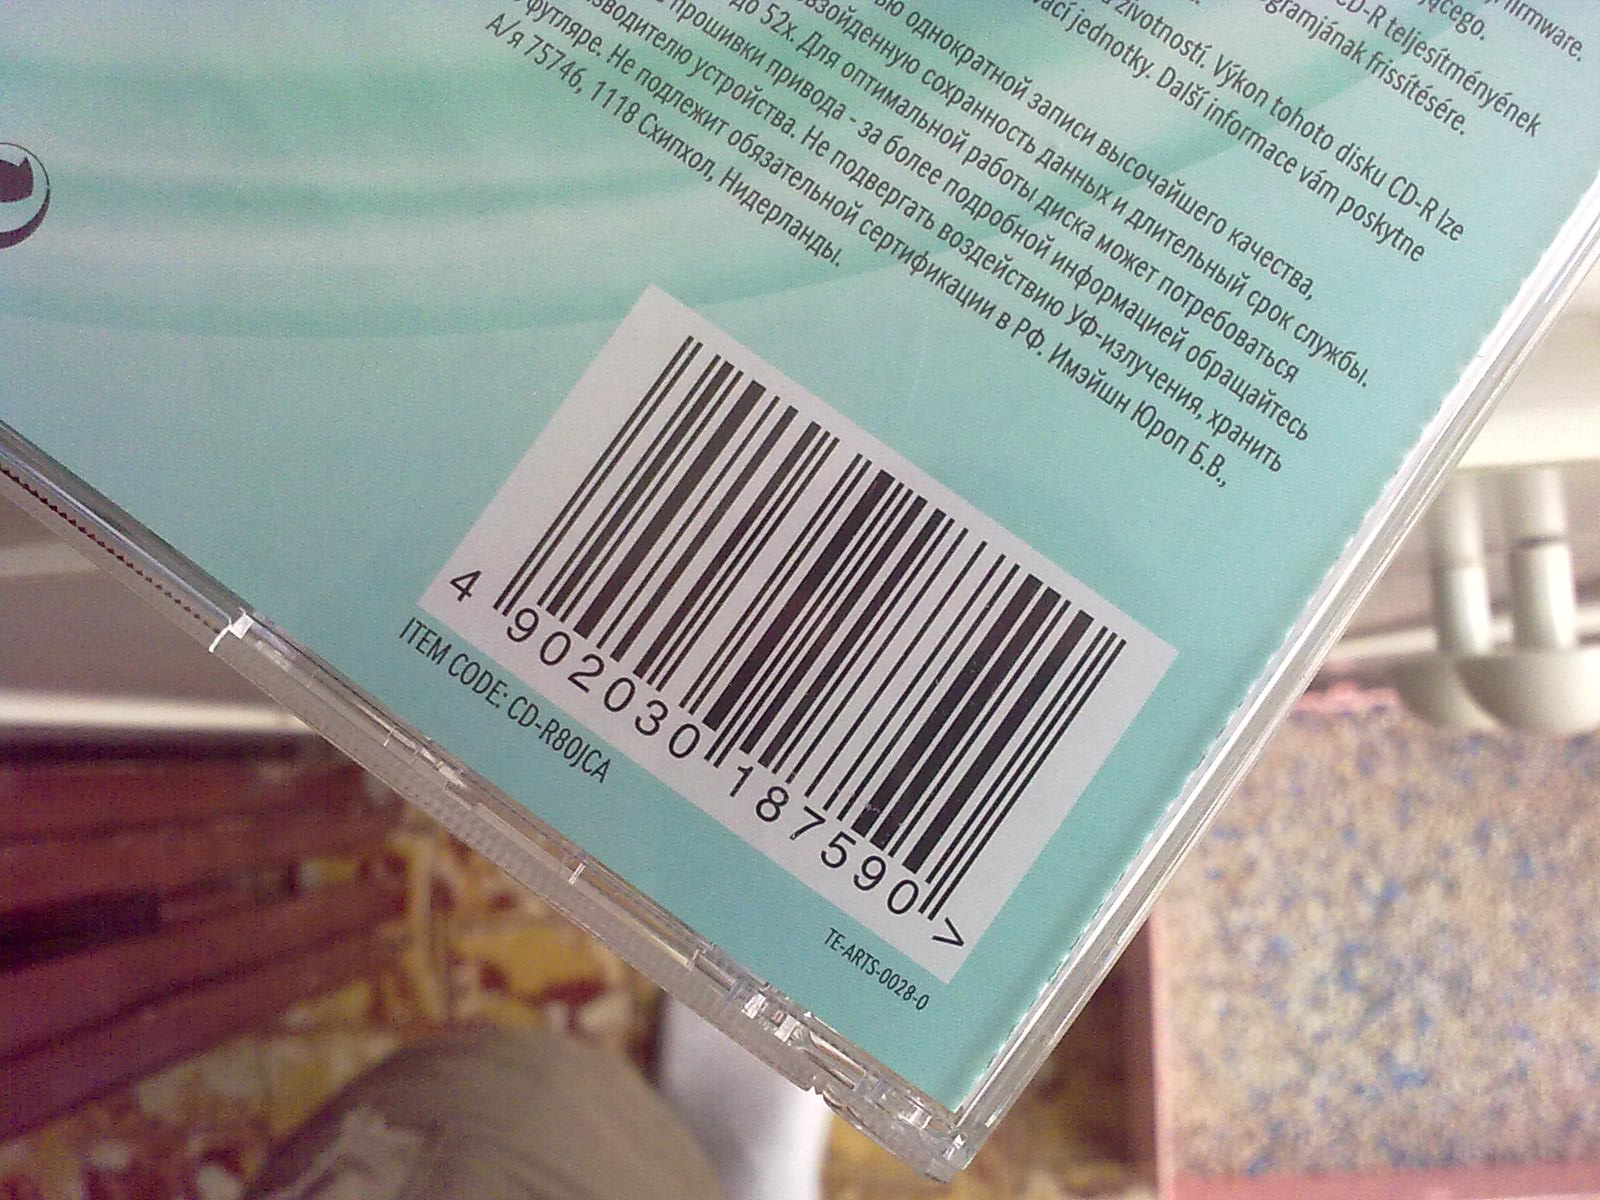
\includegraphics[width=0.5\textwidth]{images/barcode0.jpg}
	\caption{Image d'un code barre}
	\label{code_barre}
\end{figure}

Avant de pouvoir lire un code barre, nous devons opérer un seuillage de l'image. Pour cela, nous utilisons la méthode d'Otsu.
Pour rappel, cette méthode repose sur le calcul d'un seuil optimal pour binariser une image en niveaux de gris.
Ce seuil est déterminé grâce à l'histogramme de l'image et sépare les pixels en deux classes distinctes : les pixels noirs et les pixels blancs.

Pour l'image en figure \ref{code_barre}, nous obtenons l'histogramme suivant :

\begin{figure}[H] 
	\centering
	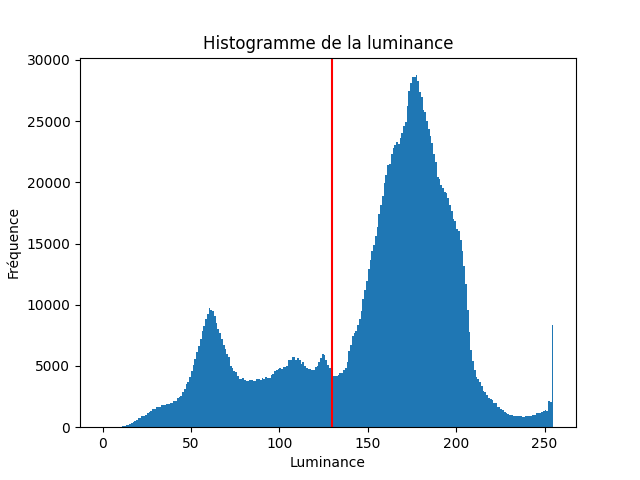
\includegraphics[width=0.5\textwidth]{images/histogramme.png}
	\caption{Histogramme de la luminance de l'image}
	\label{histogramme}
\end{figure}

Grâce à ce seuil dénoté par la barre rouge, nous obtenons ainsi l'image seuillée : 
\begin{figure}[H] 
	\centering
	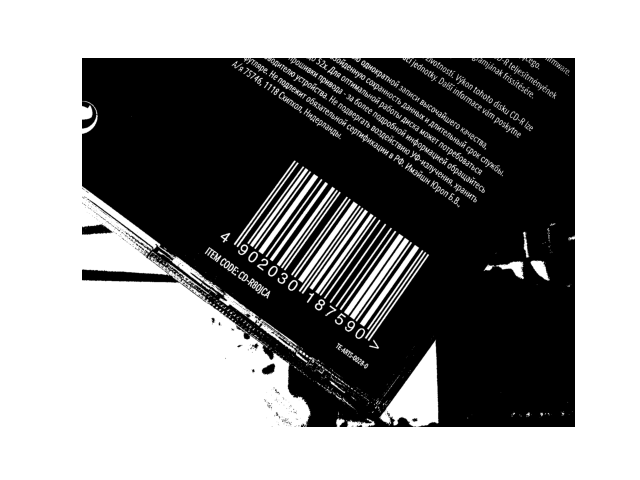
\includegraphics[width=0.5\textwidth]{images/barcode_seuillee.png}
	\caption{Image seuillée}
	\label{img_seuillee}
\end{figure}

\subsubsection*{Détermination des limites du code-barres}
Une fois le seuil déterminé, nous pouvons déterminer les limites du code barre.
La première étape consiste à un échantillonnage sur un segment puis une binarisation selon un seuil. Ce segment est visble en vert sur la figure suivante.

Nous recevons en argument deux points, qui définissent un segment sur l'image seuillée, comme représenté sur la figure \ref{fig:segment}.
Nous souhaitons alors réduire ce segment pour ne garder que les deux points correspondant à la première barre noire du code barre.

% TODO : changer les images en images seuillées
\begin{figure}[H] 
	\centering
	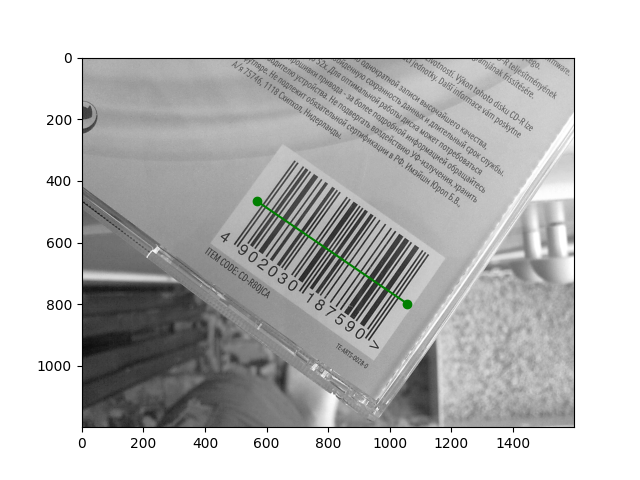
\includegraphics[width=0.5\textwidth]{images/code_barre_couple_vert.png}
	\caption{Segment défini par le deux points en arguments}
	\label{fig:segment}
\end{figure}

Ensuite, la recherche des limites du code-barres amènent à un nouveau segment entre les deux limites. 
Nous obtenons alors le nouveau segment entre les points en rouge sur l'image seuillée, comme illustré sur la figure \ref{fig:binarisation} : 

\begin{figure}[H] 
	\centering
	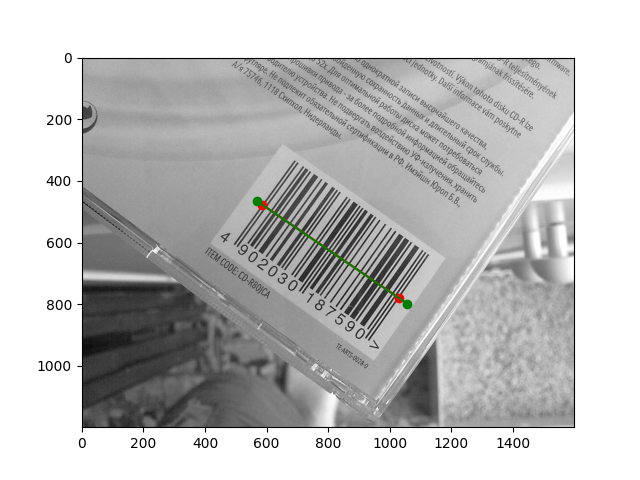
\includegraphics[width=0.5\textwidth]{images/binarisation.png}
	\caption{Nouveau segment produit par l'échantillonnage et la binarisation}
	\label{fig:binarisation}
\end{figure}

Celle-ci montre l'efficacité
de la recherche de limites qui correspondent bien à celles observables sur l'image ci-dessus.

\subsubsection*{Analyse du code barre binaire}

On en déduit alors une liste de valeurs binaires. Ceci nous permet ainsi de détecter les zones noires et blanches du code-barres. 
La figure \ref{fig:detection} illustre cette détection, où les zones noires sont représentées en rouge et les zones blanches en bleu.

\begin{figure}[H] 
	\centering
	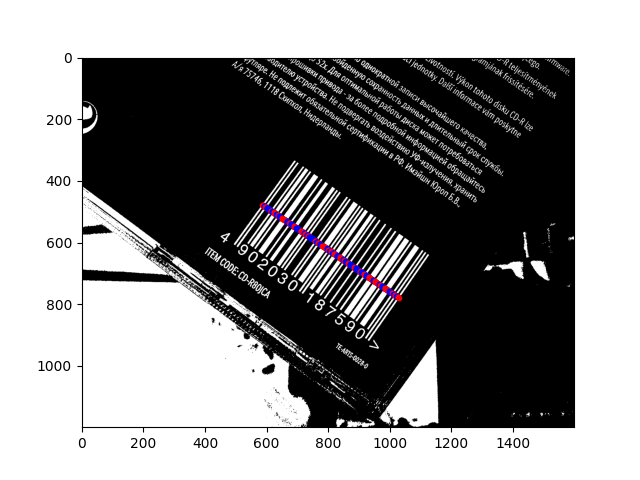
\includegraphics[width=0.5\textwidth]{images/code_seuille_couleur.png}
	\caption{Détection du noir et blanc}
	\label{fig:detection}
\end{figure}

Nous notons ici que le décalage apparent sur l'image n'est que le résultat du dé-zoom de l'image.
À petite échelle, on voit clairement que les zones sont bien détectées (cf Figure \ref{fig:detection_zoom}). 

\begin{figure}[H] 
	\centering
	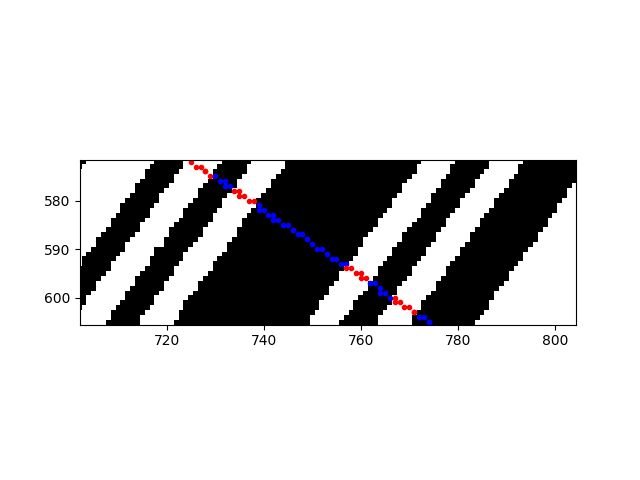
\includegraphics[width=0.5\textwidth]{images/zoom_code_seuille_couleur.png}
	\caption{Zoom de la détection}
	\label{fig:detection_zoom}
\end{figure}

\subsubsection*{Détermination du premier chiffre du code barre}
À l'aide de la séquence AB obtenue, nous pouvons ainsi déterminer le premier chiffre du code barre en se référant au tableau \ref{tab:sequence}.
En l'occurrence, nous obtenons le chiffre \textbf{4} comme premier chiffre. 

\subsubsection*{Vérification de la clef de contrôle}
Nous obtenons alors pour cette image le code \textbf{4902030187590}, ce qui correspond bien au code barre présent sur l'image (cf Figure \ref{code_barre}).
De manière générale, il faut tout de même vérifier la validité du code barre. Pour cela, nous suivons l'algorithme de vérification de code barre grâce à la clé de contrôle.

En l'occurrence, le complément à 10 du dernier chiffre du code barre vaut 0, tandis que le chiffre des unités de la somme des chiffres de rang impair et trois fois la somme des chiffres de rang pair vaut 0. 
Le code barre est donc valide.


\newpage 

\section{Conclusion}

\section{Bilan de l'organisation}

\subsection{Séance 1}

\begin{table}[H]
	\centering 
	\begin{tabular}{c|c|c}
		& Tâches entreprises& Temps passé\\ \hline
		Elisa& Prise de connaissance du sujet et commencement de la méthode d'Otsu& 2h\\ \hline
		Alban& Lecture et analyse du sujet et début de l'implémentation d'algorithme d'échantillonnage et de binarisation& 2h\\ \hline
		Tierno& & \\ \hline
		David& & 
	\end{tabular}
	\caption{Organisation de la séance 1}
\end{table}

\subsection{Séance 2}

\begin{table}[H]
	\centering 
	\begin{tabular}{c|c|c}
		& Tâches entreprises& Temps passé\\ \hline
		Elisa& Finition de la méthode d'Otsu & 2h\\ \hline
		Alban& Complétion de l'échantillonnage et de la binarisation, début du calcul des limites du code-barres et de la recherche de u& 2h\\ \hline
		Tierno& & \\ \hline
		David& & 
	\end{tabular}
	\caption{Organisation de la séance 2}
\end{table}

\subsection{Séance 3}

\begin{table}[H]
	\centering 
	\begin{tabular}{c|c|c}
		& Tâches entreprises& Temps passé\\ \hline
		Elisa& Débuggage et mise en commun de toutes les fonctions de la phase 1 & 3h\\ \hline
		Alban& Débuggage des fonctions de décodage des blocs fait chez soi et mise en commun du travail phase1& 3h\\ \hline
		Tierno& & \\ \hline
		David& & 
	\end{tabular}
	\caption{Organisation de la séance 3}
\end{table}

\subsection{Séance 4}

\begin{table}[H]
	\centering 
	\begin{tabular}{c|c|c}
		& Tâches entreprises& Temps passé\\ \hline
		Elisa& & \\ \hline
		Alban& Dernier débuggage et test sur des exemples pour vérifier l'efficacité du code& 3h\\ \hline
		Tierno& & \\ \hline
		David& & 
	\end{tabular}
	\caption{Organisation de la séance 4}
\end{table}

\subsection{Séance 5} % 13 Décembre 

\begin{table}[H]
	\centering 
	\begin{tabular}{c|c|c}
		& Tâches entreprises& Temps passé\\ \hline
		Elisa& Rédaction du rapport & \\ \hline
		Alban& Rédaction du rapport & \\ \hline
		Tierno& & \\ \hline
		David& & 
	\end{tabular}
	\caption{Organisation de la séance 5}
\end{table}

\newpage

\section{Annexes}

\lstset{style=mystyle}

\subsection{Méthode d'Otsu}
\begin{multicols}{2}
	\begin{lstlisting}
		def otsu(img, bins=255, displayHisto=False):
		luminance = None
		
		# Si l'image est en couleur (3 dimensions)
		if len(img.shape) == 3 and img.shape[2] > 1:
			# Calcul de la luminance 
			luminance = np.array([[(img[i][j][0] + img[i][j][1] + img[i][j][2])//3 for j in range(img.shape[1])] for i in range(img.shape[0])])
			luminance = luminance.ravel()
		else:
			luminance = img.ravel()
		
		# Création de l'histogramme
		histogram, bin_edges = np.histogram(luminance.ravel(), range=(0, 255), bins=bins)
		
		# Moyenner l'histogramme
		histogram = histogram/sum(histogram)    
		
		# Création d'un dico pour associer chaque valeur de luminance à sa fréquence
		histogram_dic = {int(bin_edges[i]): histogram[i] for i in range(len(histogram))}
		
		# Initialisation des moyennes et poids initiaux
		n = len(histogram_dic)
		sumB = 0
		wB = 0
		maximum = 0.0
		sum1 = sum(i * histogram_dic[i] for i in range(n))
		total = sum(histogram_dic.values())
		level = 0
		for k in range(1, n):
			wF = total - wB
			if wB > 0 and wF > 0:
				mF = (sum1 - sumB) / wF
				val = wB * wF * (sumB / wB - mF) * (sumB / wB - mF)
				
				if val >= maximum:
					level = k
					maximum = val
			
			wB += histogram_dic[k]
			sumB += (k-1) * histogram_dic[k]
		
		# Afficher l'histogramme
		if displayHisto:
			plt.figure()
			plt.hist(luminance, bins=bins, range=(0, 255))
			plt.axvline(level, color='r')
			plt.title("Histogramme de la luminance")
			plt.xlabel("Luminance")
			plt.ylabel("Fréquence")
			plt.show()
		
		return level
	
	\end{lstlisting}
\end{multicols}

\end{document}